
\documentclass[a4paper,11pt]{article}

\usepackage[british]{babel}
\usepackage[T1]{fontenc}
\usepackage[utf8]{inputenc}
\usepackage{geometry}
\usepackage{amsmath,amssymb}
\usepackage{siunitx}
\usepackage{graphicx}
\usepackage{booktabs}
\usepackage{hyperref}
\usepackage{algorithm}
\usepackage[noend]{algpseudocode}
\usepackage{tikz}
\usetikzlibrary{arrows.meta,shapes.geometric,shapes.misc,positioning}

\tikzset{
  >={Stealth},
  proc/.style = {rectangle, rounded corners, draw, align=left, minimum height=8mm, text width=35mm, align=center},
  meas/.style    = {trapezium, trapezium left angle=70, trapezium right angle=110, draw, align=left, minimum height=8mm, text width=19mm, align=center},
  decision/.style = {diamond, aspect=2.2, draw, align=center, inner xsep=1.2ex, inner ysep=1ex, text width=2cm},
  smldec/.style = {diamond, aspect=2.2, draw, align=center, inner xsep=1.2ex, inner ysep=1ex, text width=19mm},
  terminator/.style = {ellipse, draw, align=center, minimum height=8mm, minimum width=16mm},
  line/.style  = {->, line width=0.6pt}
}

\geometry{margin=1in}
\hypersetup{hidelinks}

\title{Wall- and Free-Stream Pressure Processing}
\author{Stanford Team}
\date{\today}

\algrenewcommand\algorithmicrequire{\textbf{Inputs:}}
\algrenewcommand\algorithmicensure{\textbf{Outputs:}}
\algrenewcommand\algorithmiccomment[1]{\hfill$\triangleright$ #1}

\begin{document}
\maketitle

\begin{abstract}
    This document formalises, in pseudocode, the processing pipeline. The pipeline estimates a frequency response  transfer function ($H$) between a reference and a treated microphone, then performs coherence-weighted Wiener inverse filtering to recover an estimate of the reference signal from the treated measurements.
\end{abstract}


\section{Notation and Inputs}
    Let $x[n]$ denote the discrete-time \emph{reference} pressure signal, and $y[n]$ the \emph{treated}, both sampled at $f_s=2_500$~Hz.

    \paragraph{Spectral definitions}
    Welch auto-spectra $S_{xx}[k]$, $S_{yy}[k]$ and cross-spectrum $S_{xy}[k]$ are computed with segment length $N_{\mathrm{seg}}=4096$, overlap $N_{\mathrm{ov}}=2048$, and a Hann window $w[\cdot]$. The magnitude-squared coherence is
    \begin{equation}
        \gamma^2[k] \;=\; \frac{|S_{xy}[k]|^2}{S_{xx}[k]\,S_{yy}[k]}\in[0,1].
    \end{equation}
    The FRF estimate is $H[k] = S_{xy}[k]/S_{xx}[k]$.

\section{Algorithms}

\begin{algorithm}
    \caption{$H$ Transfer-Function Estimation}
    \label{alg:H}
    \begin{algorithmic}[1]
        \Require Time series $x[n]$ (reference), $y[n]$ (treated), sampling rate $f_s$; Welch parameters $N_{\mathrm{seg}}, N_{\mathrm{ov}}, w[\cdot]$.
        \Ensure Frequency vector $f[k]$; complex FRF $H[k]$; coherence $\gamma^2[k]$.
        % \State Optionally de-mean $x$ and $y$.
        \State Compute $S_{xx}[k]$ and $S_{yy}[k]$ using Welch's method with $(N_{\mathrm{seg}}, N_{\mathrm{ov}}, w)$.
        \State Compute cross-spectrum $S_{xy}[k]$ using the same Welch settings.
        \State $H[k] \gets S_{xy}[k]/S_{xx}[k]$.
        \State $\gamma^2[k] \gets \frac{|S_{xy}[k]|^2}{S_{xx}[k]\,S_{yy}[k]}$, clipped to $[0,1]$.
        \State Return $(f[k], H[k], \gamma^2[k])$.
    \end{algorithmic}
\end{algorithm}

\begin{algorithm}
    \caption{Coherence-weighted Wiener Inverse ($\gamma^2/H$)}
    \label{alg:inv}
    \begin{algorithmic}[1]
        \Require $y_r$, sampling rate $f_s$, freq. grid $f$, transfer $H(f)$, coherence $\gamma^2(f)$%, optional band $B=[f_\ell,f_h]$
        \Ensure $\hat{x}$
        % \State $y \gets y - \mathrm{mean}(y)$
        \State $\hat{y_r} \gets \mathcal{F}(y_r, N_{\mathrm{fft}})$
        \State $m \gets |H|$;\quad $\phi \gets \mathrm{unwrap}(\angle H)$
        \State $m_i \gets \mathrm{interp}_{f\to f_r}(m)$;\quad $\phi_i \gets \mathrm{interp}_{f\to f_r}(\phi)$;\quad $H_i \gets m_i\,e^{j\phi_i}$
        \State $\gamma_i^2 \gets \mathrm{clip}\!\big(\mathrm{interp}_{f\to f_r}(\gamma^2),\,0,\,1\big)$
        \State $\varepsilon \gets \text{machine epsilon}$;\quad $H_{\mathrm{inv}} \gets \gamma_i^2 \cdot H_i^{\!*} / \max(m_i^2,\varepsilon)$
        % \If{$B$ given} \State $H_{\mathrm{inv}} \gets H_{\mathrm{inv}} \cdot \mathbf{1}_{[f_\ell,f_h]}(f_r)$ \EndIf
        \State $H_{\mathrm{inv}}[0] \gets 0$
        \State $\hat{x} \gets \mathcal{F}^{-1}\!\big(\hat{y_r} \cdot H_{\mathrm{inv}}, N_{\mathrm{fft}}\big)[0{:}N]$
        \State \Return $y$
    \end{algorithmic}
\end{algorithm}

\begin{figure}
    \centering
    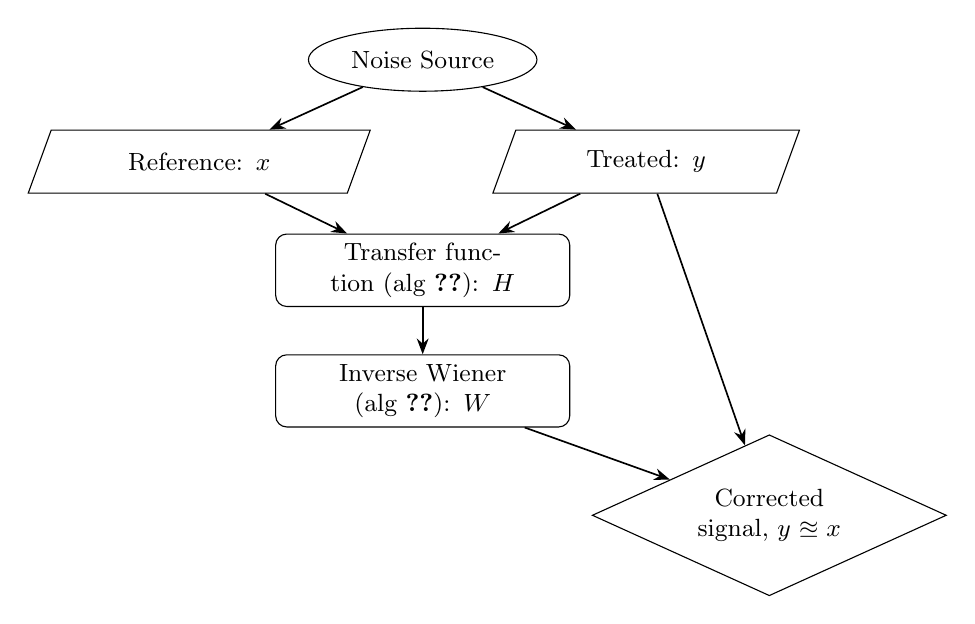
\begin{tikzpicture}[node distance=6mm and 18mm, every node/.style={font=\small}]{Generic Transfer Function}
    \title{Generic Transfer Function}
        % \centering
    % Start
        \node (start) [terminator] {Noise Source};

        % Two separate measurement boxes
        \node (ref)   [meas, below left = 6mm and 14mm of start, anchor=north east]
            {Reference: $x$};
        \node (treat) [meas, below right = 6mm and 14mm of start, anchor=north west]
            {Treated: $y$};

        \node (H)  [proc, below=18mm of start]
            {Transfer function (alg~\ref{alg:H}): $H$};

        \node (wien)  [proc, below=of H]
            {Inverse Wiener (alg~\ref{alg:inv}): $W$};

        \node (corr)  [decision, below right = 6mm and 14mm of wien]
            {Corrected signal, $y \approxeq x$};

        \draw [line] (start) -- (ref);
        \draw [line] (start) -- (treat);
        \draw [line] (ref) -- (H);
        \draw [line] (treat) -- (H);
        \draw [line] (H) -- (wien);
        \draw [line] (wien) -- (corr);
        \draw [line] (treat) -- (corr);

    \end{tikzpicture}
    \caption{Generic transfer function processing pipeline.}
\end{figure}

\begin{figure}
    \centering
    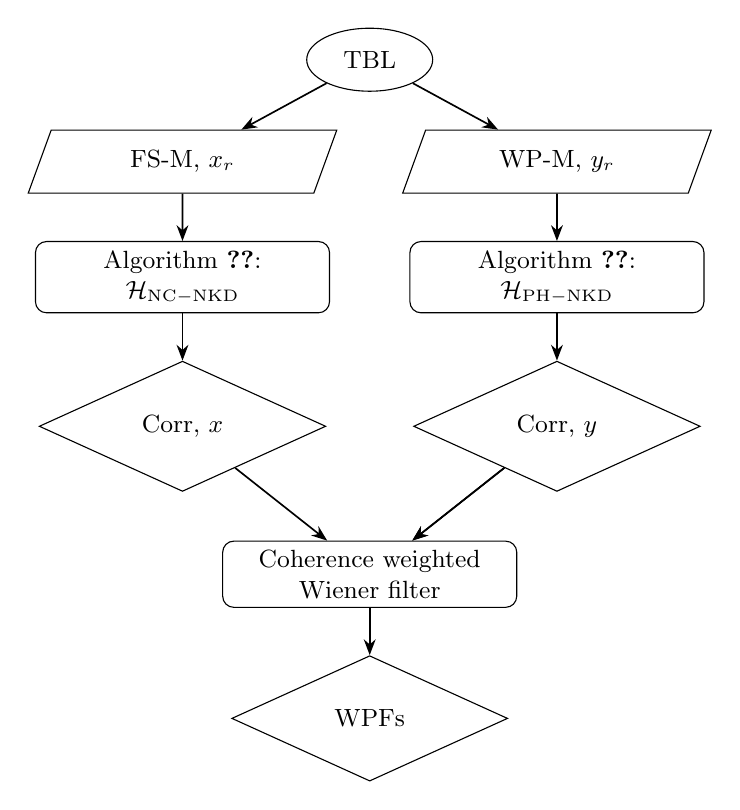
\begin{tikzpicture}[node distance=6mm and 18mm, every node/.style={font=\small}]
        \centering
    % Start
        \node (start) [terminator] {TBL};

        % Two separate measurement boxes
        \node (refraw)   [meas, below left = 6mm and 14mm of start, anchor=north east]
            {FS-M, $x_r$};

        \node (Href) [proc, below=of refraw]
            {Algorithm~\ref{alg:inv}: $ \mathcal{H}_{\mathrm{NC-NKD}}$};

        \node (ref) [decision, below=of Href]
            {Corr, $x$};

        \node (tretraw) [meas, below right = 6mm and 14mm of start, anchor=north west]
            {WP-M, $y_r$};

        \node (Htret)  [proc, below=of tretraw]
            {Algorithm~\ref{alg:inv}: $\mathcal{H}_{\mathrm{PH-NKD}}$};

        \node (tret)  [decision, below=of Htret]
            {Corr, $y$};

        \node (corr)  [proc, below=57mm of start]
            {Coherence weighted Wiener filter};

        \node (post)  [decision, below=of corr]
            {WPFs};

        \draw [line] (start) -- (refraw);
        \draw [line] (refraw) -- (Href);
        \draw [line] (Href) -- (ref);
        \draw [line] (start) -- (tretraw);
        \draw [line] (tretraw) -- (Htret);
        \draw [line] (Htret) -- (tret);
        \draw [line] (tret) -- (corr);
        \draw [line] (ref) -- (corr);
        \draw [line] (tret) -- (corr);
        \draw [line] (corr) -- (post);

    \end{tikzpicture}
    \caption{Complete pressure processing pipeline for measurement of the WPFs through a pinhole microphone.}
\end{figure}

\begin{algorithm}[H]
    \caption{Two-microphone Wiener noise cancellation for wall pressure}
    \begin{algorithmic}[1]
        \Require Wall mic $y[0{:}N\!-\!1]$, free-stream mic $r[0{:}N\!-\!1]$, sampling rate $f_s$
        \Ensure Estimate of true wall pressure $\widehat{x}$
        \State $y \gets y - \mathrm{mean}(y)$;\quad $r \gets r - \mathrm{mean}(r)$
        \State Estimate spectra via Welch: $S_{rr}(f)$ and $S_{yr}(f)$ \Comment{$S_{yr}$ is cross-PSD}
        \State $F(f) \gets \dfrac{S_{yr}(f)}{S_{rr}(f)+\varepsilon}$ \Comment{Wiener filter mapping $r \to y$}
        \State $R(f) \gets \mathrm{rFFT}(r)$;\quad $Y(f) \gets \mathrm{rFFT}(y)$
        \State $\widehat{D}(f) \gets F(f)\,R(f)$ \Comment{Predicted free-stream noise at wall mic}
        \State $\widehat{X}(f) \gets Y(f) - \widehat{D}(f)$
        \State $\widehat{x} \gets \mathrm{irFFT}\!\left(\widehat{X}(f)\right)$
        \State \Return $\widehat{x}$
    \end{algorithmic}
\end{algorithm}

\end{document}